\chapter{Results - Sliding Puzzle} % Main chapter title

\label{sec:ResultsSP} % Change X to a consecutive number; for referencing this chapter elsewhere, use \ref{ChapterX}


In this chapter, I show and discuss results on \textbf{SP} of various dimensions, going from \textit{small} dimensions (which I define as those I can reasonably \textit{fully} solve given my computing resources, the finite time I have to complete this project, and the choice of programming language), then I move to studying in much detail the case of the 3x3, and finally move on to slightly higher dimensions 3x4 and 4x4. Table \ref{tab:gridSP} below shows which solvers I have run on each of the dimensions attempted. The reader is referred to the implementation chapter \ref{sec:Implementation} for a detailed explanation of each of these solvers, and to the appendix section \ref{sec:Examples} for code examples on how to run them.

\begin{table}[H]
\begin{center}
\begin{tabular}{l*{9}{c}r}
\hline
\textbf{solver}      & & \textbf{Sliding Puzzle} & \textbf{2x2} & \textbf{2x3} & \textbf{2x4} & \textbf{2x5}  & \textbf{3x3} & \textbf{3x4} & \textbf{4x4} \\ 
\hline
BFS   & & & & & & &  x  & & \\
\hline
A$^{*}$[Manhattan]   & & & & & &  x  &  x  &  x  & \\
\hline
A$^{*}$[Manhattan++]   & & & & & &  x  &  x  &  x  & x \\
\hline
A$^{*}$[Perfect]   & & &  x  &  x  &  x  &  x  &  x  & & \\
\hline
Naive   & & & & & & &  x  &  x  & x \\
\hline
A$^{*}$[DL[FullyConnected]]   & & & & & & &  x  &  x  & x \\
\hline
A$^{*}$[DL[Convolutional]]   & & & & & & &  x  &  & \\
\hline
A$^{*}$[DRL]   & & & & & & &  x  &  x  & x \\
\hline
A$^{*}$[DQL]   & & & & & & &  x  & & \\
\hline
MCTS[DQL]        & & & & & & &  x  & & \\
\end{tabular}
\caption{\label{tab:gridSP} Solvers used vs \textbf{SP} dimension}
\end{center}
\end{table}

\noindent I am neither making claims of depth (each solver could surely be tuned and optimized/adapted, possibly differently for each dimension) nor breadth (I have not run all of the solvers versus each dimension). Running these experiments takes a lot of computing time (even though I have very decent computing resources), so I had to be somewhat selective. I wanted however to run all of the solvers I have implemented one one particular dimension (the intermediary 3x3 seemed appropriate to do so) and try to answer as many of the following interesting questions as possible:
\begin{itemize}
\item How hard is too hard for \textbf{BFS} to complete in \textit{reasonable} time?
\item How much, if any, improvement do we get with Manhattan++ over Manhattan?
\item Is there much loss between \textbf{DL} and \textbf{DRL}, i.e. is losing the teacher used by \textbf{DL} a deal breaker?
\item Is \textbf{DQL}, all things being equal, able to learn a better cost-to-go heuristic than \textbf{DRL}?
\item How does \textbf{MCTS} perform? How important is it to tune the hyper-parameter $c$? How much improvement, if any, does the post trim of the \textbf{MCTS} tree via \textbf{BFS} bring?
\item Are any of the \textbf{D*L} techniques able to perform on par with A$^{*}$ with Manhattan++ or perfect heuristic?
\end{itemize}
All of these questions are answered (obviously not in generality, but in the context of the experiments I have been running) in this chapter.











%----------------------------------------------------------------------------------------
%	SECTION 1
%----------------------------------------------------------------------------------------

\Section{Low dimension}
\label{sec:SPLowDimension}

\Subsection{God numbers and hardest puzzles}

As mentioned in chapter \ref{sec:Puzzles}, the state space cardinality for the \textbf{SP} grows very quickly with n and m. The only dimensions which have less than 239.5 millions states are shown in table \ref{tab:smallSP}. Note I am also only considering n $\leq$ m since dimension mxn can always be solved by symmetry from the solutions mxn:

\begin{table}[H]
\begin{center}
\begin{tabular}{l*{6}{c}r}
n              & m & 2 & 3 & 4 & 5\\
\hline
2              &   & 12 & 360 & 20,160 & 1,814,400 \\
3              &   &   & 181,440 &  &    \\
\end{tabular}
\caption{\label{tab:smallSP}\# puzzles for \textit{small} dimensions}
\end{center}
\end{table}
\noindent In this section, I will discuss \textit{full} results for these 5 dimensions. In order to fully solve them, one can simply use rubiks.scripts.learner, setting up the PerfectLearner with A* and manhattan heuristic, or instantiate directly a PerfectLearner as have seen in section \ref{PLSS}. I obtained the following God numbers (table \ref{tab:smallSPGN}) for these puzzles:
\begin{table}[H]
\begin{center}
\begin{tabular}{l*{6}{c}r}
n              & m & 2 & 3 & 4 & 5\\
\hline
2              &   & 6 & 21 & 36 & 55* \\
3              &   &   & 31 &  &    \\
* \tiny{provisional result}
\end{tabular}
\caption{\label{tab:smallSPGN}God numbers for \textit{small} dimensions}
\end{center}
\end{table}
\noindent Among the above dimensions, 2x5 has the largest state space. My current result in table \ref{tab:smallSPGN} for that dimension is provisional, as I have only solved about 1.2 million puzzles out of the 1.8 million possible configurations, despite running a combined 600 hours (most of the time over 16 cores, except for a full week-end run on a 72-core c5.18xlarge Amazon EC2 instance). It is well possible that I haven't yet bumped into the hardest configuration though!
\\
\\
The perfectLearner also keeps track of the hardest puzzle it has encountered (i.e. a configuration whose optimal solution has a cost equal to the God number). I obtained the following hardest puzzles for each of the 5 \textit{small} dimensions:
\\
\begin{three}
\centering
\setrow{2}{,3}
\setrow{1}{2,1}
\end{three}
\begin{five}
\setrow{2}{4,5,}
\setrow{1}{1,2,3}
\end{five}
\begin{seven}
\setrow{2}{,7,2,1}
\setrow{1}{4,3,6,5}
\end{seven}
\begin{nine}
\setrow{2}{,9,3,7,1}
\setrow{1}{5,4,8,2,6}
\end{nine}
\begin{eight}
\setrow{3}{8,6,7}
\setrow{2}{2,5,4}
\setrow{1}{3,,1}
\end{eight}


\Subsection{Manhattan heuristic}
\label{MHComp}
In this section, I verify empirically that, as expected, the overhead of adding penalty in Manhattan++ for the linear constraint (which have all been precomputed and stored in a database) is more than compensated for by the reduction in nodes expansion. I have run my solver script for 2x5 in performance test mode, for both Manhattan and Manhattan++, with 250 randomly shuffled puzzles with \textit{nb\_shuffles} from 0 to 60 by increment of 5, as well as with \textit{nb\_shuffles = $\inf$}. The resulting run time and nodes expansions are as follows:

\begin{figure}[H]
\centering
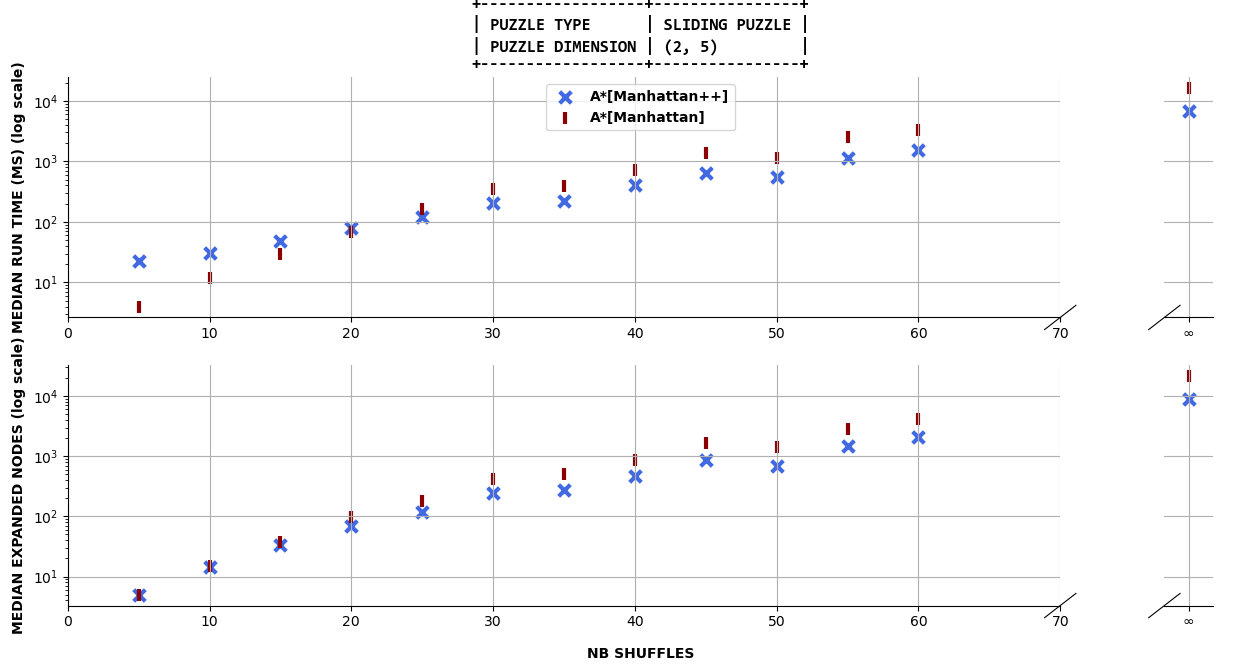
\includegraphics[scale=0.40]{./Figures/25SPPerformanceManhattan}
\caption[SP]{Manhattan vs Manhattan++ for the 2x5 \textbf{SP}}
\label{fig:25SPPerformanceManhattan}
\end{figure}

\noindent As can be seen, for low difficulty (up to \textit{nb\_shuffles = 20}), the node expansions are about the same in both cases, and the overhead of adding the linear constraints penalty increases the run time. However, for any non trivial case, Manhattan++ outperforms considerably (by a factor of about 2.5). Table \ref{tab:mppOutperformance} below summarizes the results for the 250 \textit{perfectly} shuffled configurations:



\begin{table}[H]
\begin{center}
\begin{tabular}{l*{7}{c}r}
                              & avg cost  & max cost & avg nodes & max nodes & avg run time (ms) & max run time (ms) \\
\hline
Manhattan                   &  34.6  & 49 & 46,483 & 575,050 & 36,088 & 428,887 \\
Manhattan++              & 34.6 &  49 & 18,780 & 213,557 & 14,665 & 165,830 \\
Improvement               & n/a &  n/a & \textbf{x2.5} & \textbf{x2.7} & \textbf{x2.5} & \textbf{x2.6} \\
\end{tabular}
\caption{\label{tab:mppOutperformance} Manhattan++ outperformance on perfectly scrambled 2x5 \textbf{SP}}
\end{center}
\end{table}






%-----------------------------------
%	SECTION 2
%-----------------------------------
\Section{Intermediary case - 3x3}
\label{sec:S33}

In this section, which focusses on the 3x3 \textbf{SP}, I detail some results from the PerfectLearner (\ref{sec:S33PL}) before moving to a discussion of the \textbf{DQL} \textbf{MCTS} solver and the effect of its trade-off hyper-parameter \textit{c} and of its optional \textbf{BFS} tree-trimming on the quality of the solutions (\ref{sec:MTCSHyperParamsEffect}). I then run a comprehensive comparison of my 10 different solvers on the 3x3 \textbf{SP} in \ref{ssec:33SPSC} including \textbf{DL},  \textbf{DRL} and  \textbf{DQL}. Finally, I end the section by running a few select solvers on one of the two hardest 3x3 puzzle in \ref{ssec:33SPHard}


\Subsection{Perfect learner}
\label{sec:S33PL}
As discussed in the previous section section \ref{sec:SPLowDimension}, the 3x3 \textbf{SP} is one of the cases I have been able to solve perfectly, since it only has 181,440 possible configurations. Its God number is only 31, which definitely makes it manageable. However, this is already an intermediary size, large enough that it is worth trying and comparing a few different methods, including \textbf{DL}, \textbf{DRL} and \textbf{DQL}. To start with, I ran the PerfectLearner and the results are shown below in figure \ref{fig:33SPPerfectLearning}. It is interesting to note that there are only two hardest configurations (of cost 31) and 221 configurations of cost 30.


\begin{figure}[H]
  \noindent
  \makebox[\textwidth]{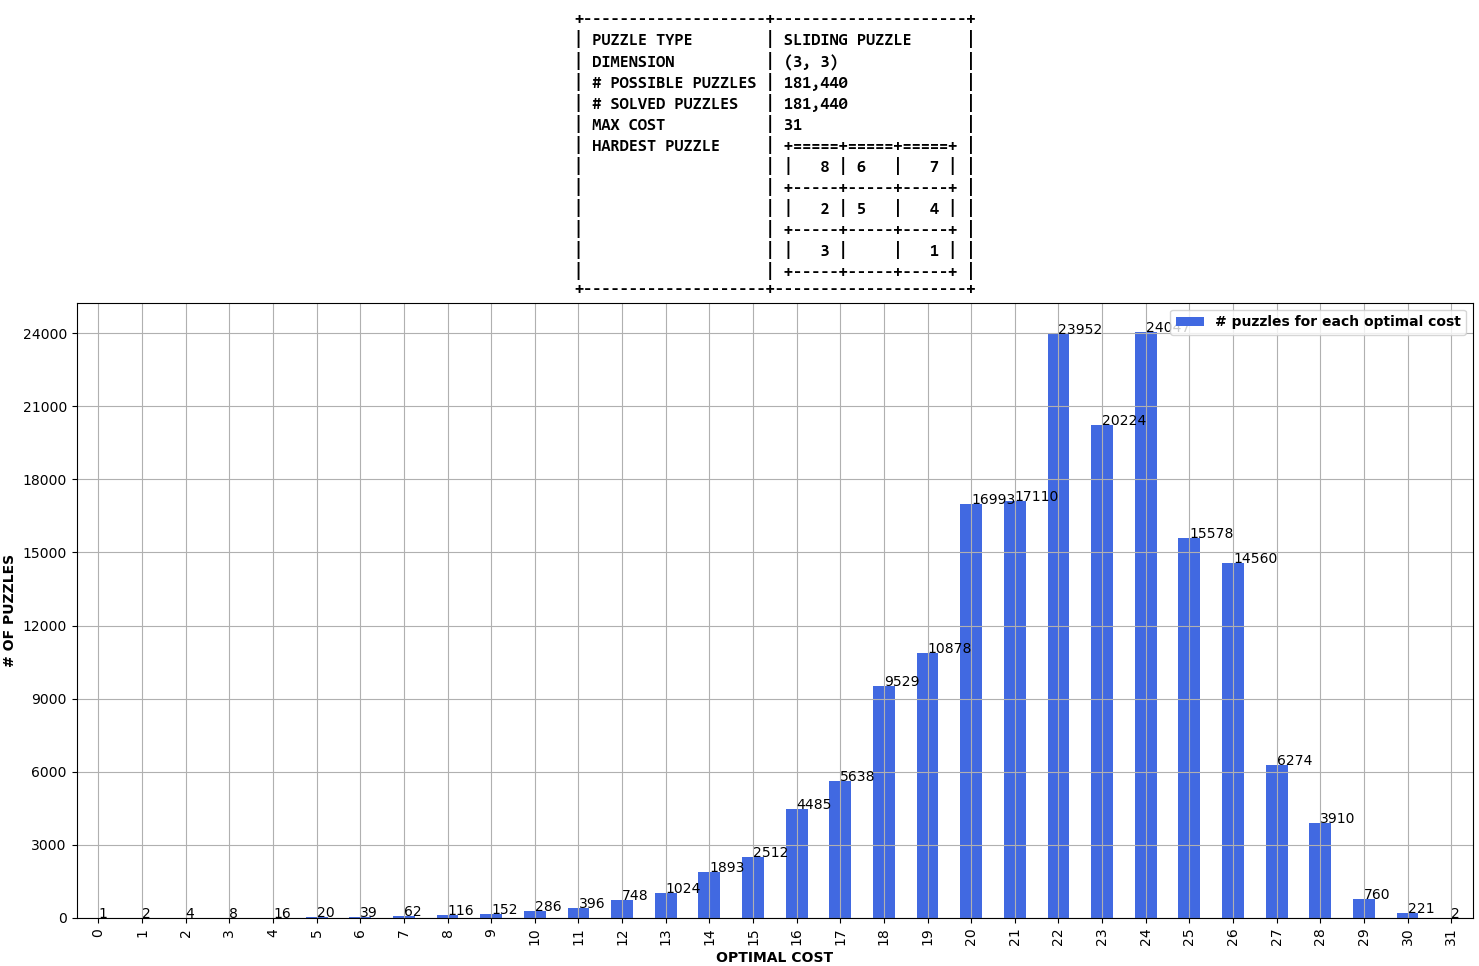
\includegraphics[scale=0.4]{./Figures/33SPPerfectLearning}}
  \caption[33SPPerfectLearning]{Perfect Learning of the 3x3 \textbf{SP}}
  \label{fig:33SPPerfectLearning}
\end{figure}




%\Subsection{Deep reinforcement learner}
%\label{sec:S33DRL}


\begin{comment} 

Next I have run the DeepReinforcementLearner with the following main parameters:
\begin{itemize}
\item Update the target network every 1,000 epochs (\textit{update\_target\_network\_frequency=1000}) or when the MSE falls below 10 basis points of the maximum target cost-to-go (\textit{update\_target\_network\_threshold=1e-3})
\item Run for a maximum of 11,000 epochs (\textit{nb\_epochs=11000}) or when the maximum target so far has not been increasing by more than 1\% in the last 5,500 epochs (\textit{max\_target\_uptick=1e-2} and \textit{max\_target\_not\_increasing\_epochs\_pct=0.5})
\item At every update of the target network (\textit{training\_data\_every\_epoch=False}), generate 100 sequences of puzzles (\textit{nb\_sequences=100}), each comprised of a 50-scramble puzzle back to goal state, with all intermediary puzzles along the path (\textit{nb\_shuffles=50}).
\item Use a fully connected network (\textit{network\_type=fully\_connected\_net}) with three hidden layers of size 600, 300, 100 (\textit{layers\_description=(600,300,100)}) and use torch.optim.RMSProp as optimiser (\textit{optimiser=rms\_prop}) with an exponential scheduler (\textit{scheduler=exponential\_scheduler}) with gamma 0.999 (\textit{gamma\_scheduler=0.9999}).
\end{itemize}
Below I show some of the DeepReinforcementLearner's quantities tracked over the epochs (see \ref{fig:33SPDeepReinforcementLearning}). I have shown only the following quantities:
\begin{itemize}
\item learning rate, which decreases due to the scheduler, but gets reset at each network update.
\item max target. One interesting dynamic during learning is that due to the way targets are constructed using value-iteration update, and starting from an all 0 network, the max target only increases by about 1 at best at every network update. That is, the first network only learns how to differentiate goal from non-goal, then the second one learns how to differentiate goals, cost 1 and cost 2+ in some sense. This is why I have introduced the first set of parameters discussed just above. The first one makes sure we do not waste time initially training the left-hand-side network when training is easy (as consist of just goal versus not goal). The second ones make sure that we stop training altogether when the max target does not grow anymore. This is because we do not know a-priori what the God number of a given puzzle/dimension is, but let's assume for the sake of the argument that it is 15. Then that means that after 15 updates of the target network we might not really get so much benefit by keeping training and value-iterating.
\item the MSE loss
\item the MSE loss divided by the max target. The exit criterion \textit{update\_target\_network\_threshold} is based on that quantity, since a loss of e.g. 0.01 means little if the we do not compare it to the possible range that the cost-to-go can take.
\item The percentage of all the possible puzzles of that dimension \textit{seen} by the DeepReinforcementLearner. This is an interesting quantity, as it tells us later on when testing out of sample and comparing with other solvers, how well the solvers are able to generalise. In this case (3x3) we can see that the DeepReinforcementLearner quickly has seen a very large percentage of all puzzles. That being said, it is good to keep in mind that \textit{seen} does not mean really much here, since the learning is unsupervised. This is quite in contrast to the DeepLearner, for which puzzles seen come along with the cost-to-go computed by a \textit{teacher}, usually an optimal or at least efficient solver.
\end{itemize}


\begin{figure}[H]
\centering
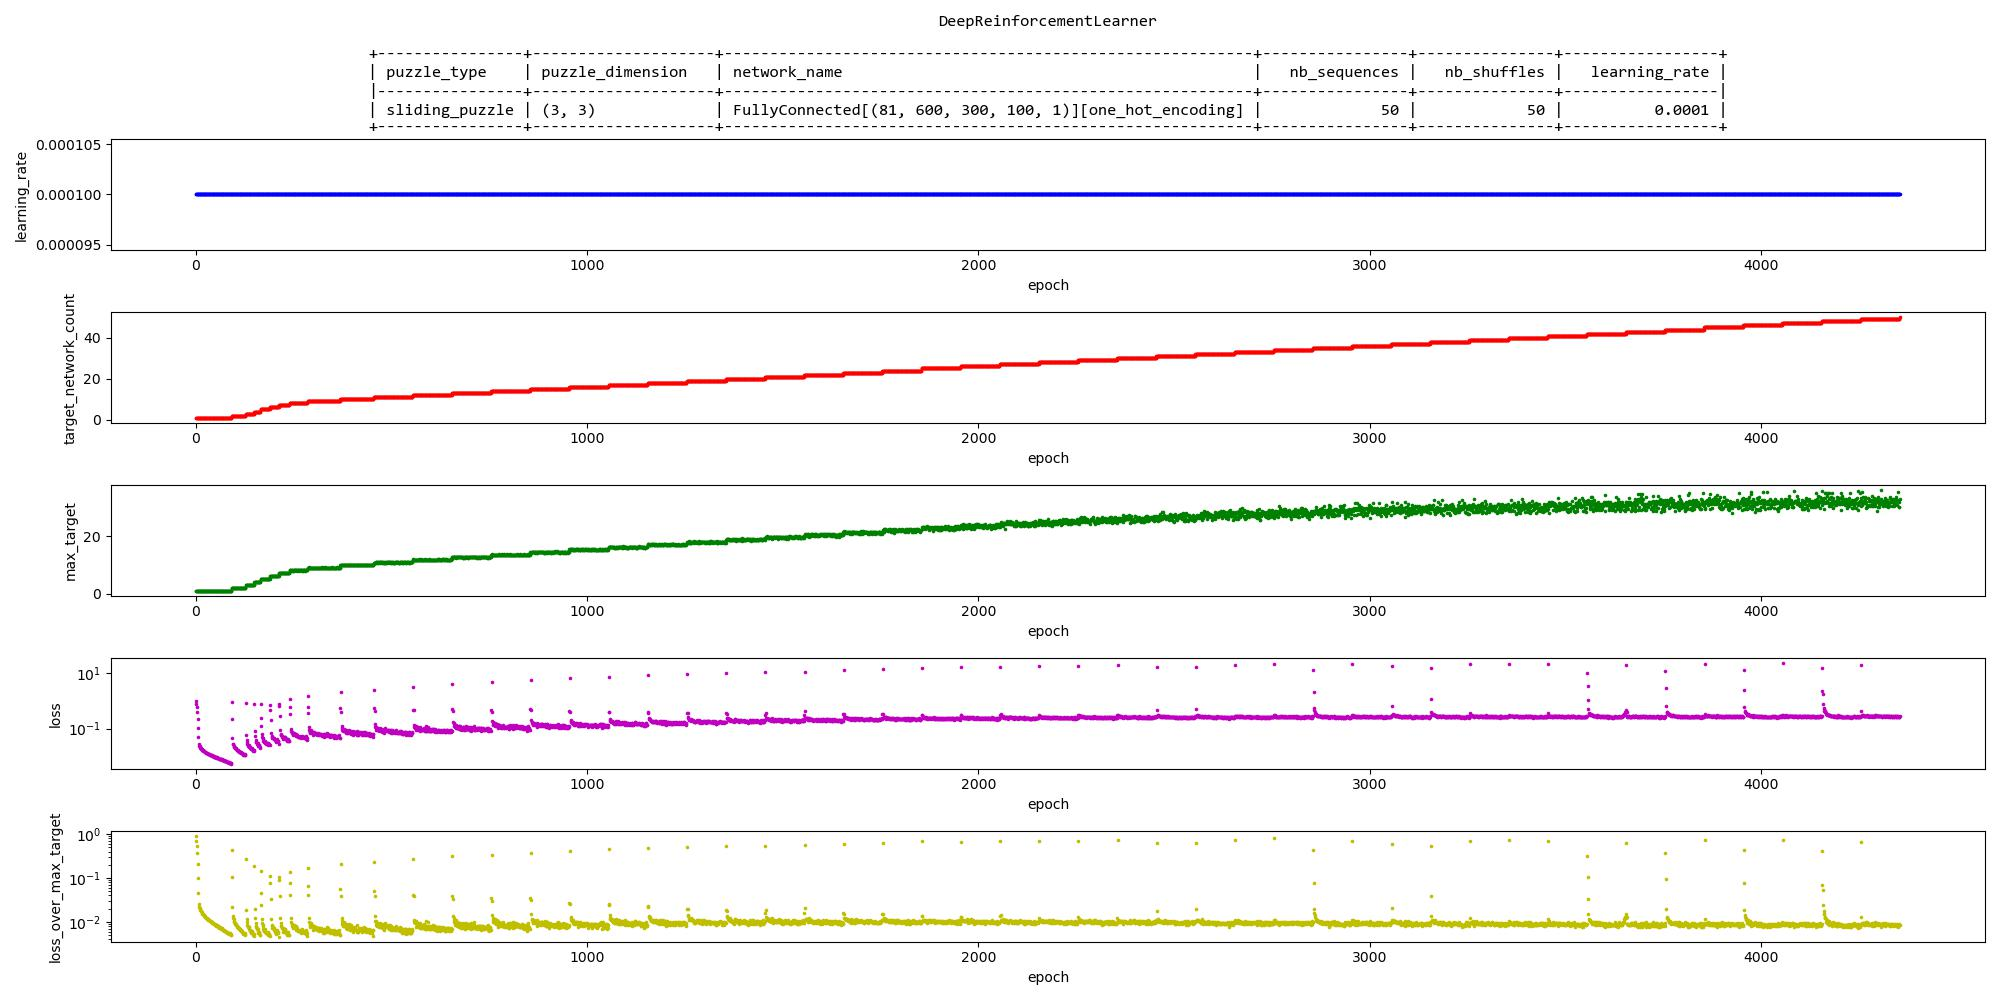
\includegraphics[align=c, scale=0.42]{./Figures/33SPDeepReinforcementLearning}
\caption[33SPDeepReinforcementLearning]{\textbf{DRL} of the 3x3 \textbf{SP}}
\label{fig:33SPDeepReinforcementLearning}
\end{figure}

Notice that the DeepLearner and DeepQLearner have very similar sets of parameters and track similar metrics during their learning for later display, but I shall not detail it here since there is not much extra insight to be had compared to the DeepReinforcementLearning example we just went through.

\end{comment} 

\Subsection{MCTS DQL}
\label{sec:MTCSHyperParamsEffect}
In this subsection I explore the effect on \textbf{MCTS} of the trade-off hyper-parameter $c$ as well as of trimming the resulting tree via \textbf{BFS}. (see the threory section \ref{sec:TheoryMCTS} as well as the implementation section \ref{sec:codesolvers} for more details). To that effect, I have run my Solver performance test with four different values of $c$ (0, 1, 10 and 100), and in each case, with and without \textbf{BFS} trimming. A$^{*}[Manhattan++]$ is also presented to have an optimal solver benchmark. For each level of difficulty, the test present the solvers with the same 150 random configurations (for fairness and to increase the significance of the results). The levels of difficulty (number of scrambles from goal) used here go from 5 to 50 in step of 5. The tests were also run with perfect shuffling (difficulty = $\infty$ on the graphs), corresponding to taking scrambling to $\infty$ as explained in \ref{Theory:SPSSS}). I used a \textit{time\_out} of 5 minutes, which none of the solvers hit on any of the (1,650) configurations they were presented with.
The detailed results (percentage of configurations solved, optimality score, median and max cost, run time and expanded nodes) are shown on the next page \ref{fig:33SPPerformanceMCTS}, but let me make here some remarks on those results:
\begin{itemize}
\item $c=0$ makes no exploration as it simply follows the path of lowest cost-to-go. As $c$ increases, we expect more exploration, and therefore higher run time, more expanded nodes, and higher quality solutions. This is what we observe, where $c=0$ converges (for difficulty=$\infty$) to solutions on average three times longer than the optimal solver but take not much longer to obtain. At the other extreme, $c=100$ takes almost 2 orders of magnitude more time to obtain a solution, but these solutions are only 20-25\% longer than that of the optimal solver
\item trimming via \textbf{BFS} takes hardly any time, and improves solutions' lengths by about 10\% at high values of $c$. At low value of $c$ there is little benefit as expected (since the trees are deep but not bushy at all and have much fewer leaves and branches).
\item The quality of solutions is not amazing, but then given the algorithm has not really any mechanism to guarantee optimality this is not very surprising. 
\item Notice that the number of expanded nodes can be compared within \textbf{MCTS} but given the algorithm is totally different to A$^{*}$ it makes little sense to compare between the different families of solvers. Also one point to note is that \textbf{MCTS} would be fairly easy to multithread (within the same process) using an appropriate language such as C++, and this is what \cite{https://doi.org/10.48550/arxiv.1805.07470} have done, and probably why they get considerably faster and better results.
\item Despite the name \textit{Monte Carlo}, there is no randomness (or even peudo-randomness) in this algorithm, since the paths generated at each iteration are really just a deterministic function of the output of the \textbf{DQL} network (or QHeuristic in my code-jargon).
\end{itemize}


\begin{figure}[H]
  \noindent
  \makebox[\textwidth]{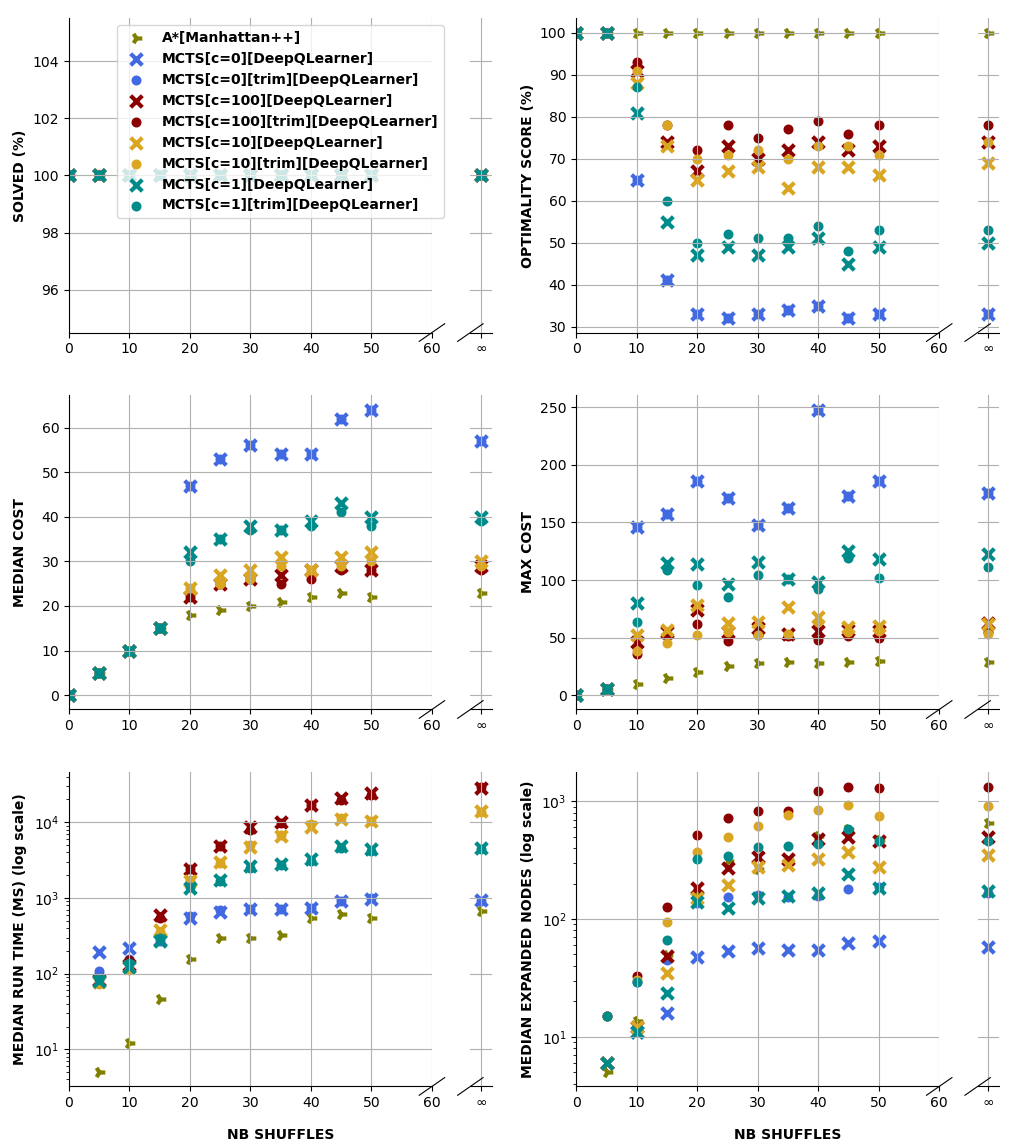
\includegraphics[scale=0.6]{./Figures/33SPPerformanceMCTS}}
\caption[33SPPerformanceMCTS]{\textbf{MCTS} tuning 3x3 \textbf{SP}}
\label{fig:33SPPerformanceMCTS}
\end{figure}



\Subsection{Solvers' comparison}
\label{ssec:33SPSC}
\label{sec:S33DRLDQL}
As promised earlier in table \ref{tab:gridSP}, I have run the Solver's comparison test with 10 different solvers (Naive, \textbf{MCTS}, \textbf{BFS}, A$^{*}$ with the following heuristics: Manhattan, Manhattan++, Perfect, \textbf{DRL}, \text{DQL} and \text{DL}), to get an idea of their respective success rate, strengths and weaknesses. The \textbf{DRL} and \textbf{DQL} heuristics were trained with the exact same parameters and a fully connected network of 3 hidden layers with 600, 300 and 100 nodes. For the \textbf{DL} heuristic (trained on perfect solutions from A$^{*}$[Perfect]) I tried with the same fully connected network as well as with a combination of parallel fully connected and convolutional layers (see figure \ref{fig:33SPnets} for the exact architecture I used). The detailed results (percentage of configurations solved, optimality score, median and max cost, run time and expanded nodes) can be found on the next page  in figure \ref{fig:33SPPerformance}. Each solver had to solve 1,000 random puzzles for each level of difficulty (scrambling from goal) going from 5 to 50 in step of 5, as well as for perfect shuffling. Let me list some of the important findings from this rather comprehensive experiment:

\begin{itemize}
\item As expected, \textbf{BFS} becomes quickly hopeless.
\item The naive solver is obvioulsy by far the fastest but finds poor solutions (about 2.5 longer on average than optimal).
\item As discussed in the previous section, \textbf{MCTS} is slow, and even with much exploration and \textbf{BFS} tree trimming found solution about 25\% longer than optimal.
\item I originally was naively hoping a pure convolutional network would do well but did not manage to get the loss to converge. I later realized that this is quite different from the typical image patterns recognition as there is less direct translation and scale invariants at play here, and decided instead to try combining convolutional with fully connected layers in parallel in order to appropriately value 2x2 patterns together with their position on the sliding-puzzle. That did improve things, but overall I saw little difference in performance from my simpler 3-hidden-layer fully connected network.
\item \textbf{DRL} and \textbf{DQL} heuristics, though not as efficient in terms node-expansion as the perfect and the \textbf{DL} heuristics, were rather surprisingly doing better than Manhattan++. They ended up \textit{seeing} around 25\% of all the possible configurations during training (in an \textit{unsupervised} way though) so did show some reasonable amount of out-of-sample generalization. Their optimality score was an impressive 99\%+ at all levels of difficuly for \textbf{DRL} and 98\%+ for \textbf{DQL}. Even more interestingly, the \textbf{DQL} heuristic expanded almost 4 times less nodes than \textbf{DRL}, suggesting some benefit from the joint learning of the policy and value function.
\item The \textbf{DL} heuristics (fully connected and convolutional) performed almost on par with the perfect heuristic (optimality score of 99\%+ at all levels of difficulty and nodes expansion only increased by about 12\%), despite seeing only 8\% of the configurations by the end of their training.
\end{itemize}


\begin{figure}
  \noindent
  \makebox[\textwidth]{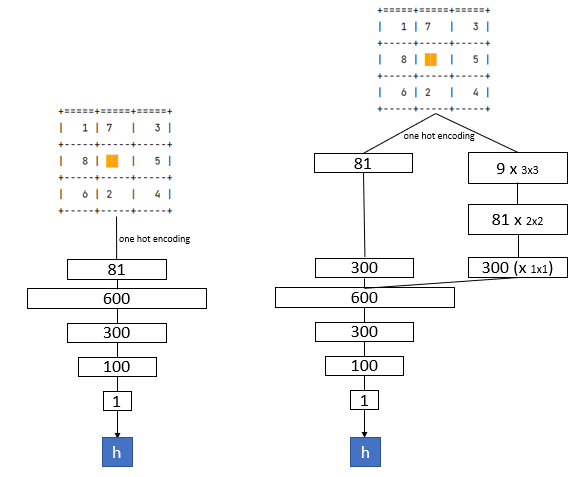
\includegraphics[scale=0.45]{./Figures/33SPnets}}
  \caption[33SPnet]{Architecture I used for the \textbf{DL} heuristics training on the 3x3 \textbf{SP}}
  \label{fig:33SPnets}
\end{figure}



\begin{figure}[H]
  \noindent
  \makebox[\textwidth]{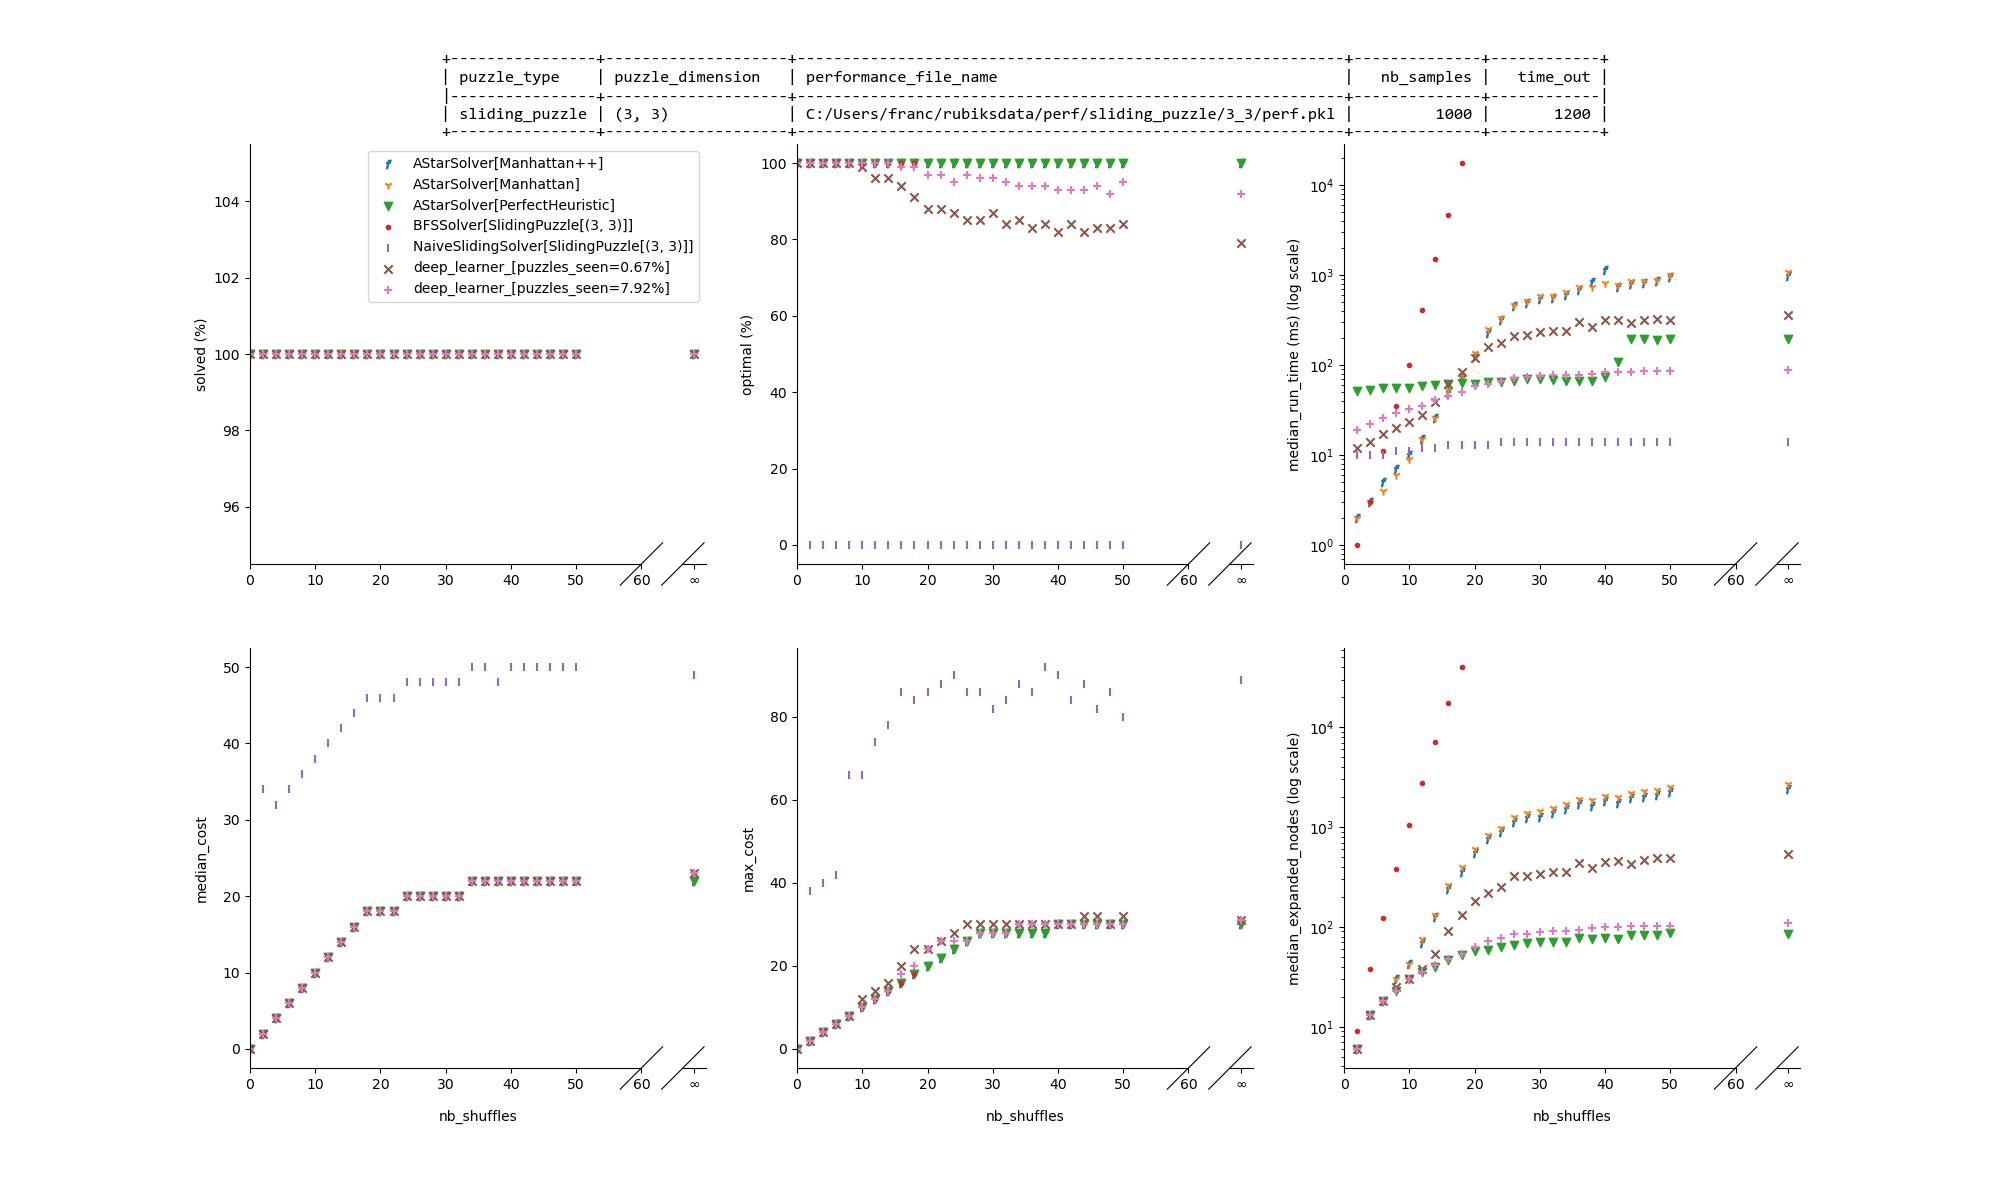
\includegraphics[scale=0.55]{./Figures/33SPPerformance}}
  \caption[33SPPerformance]{Solvers' performance comparison 3x3 \textbf{SP}}
  \label{fig:33SPPerformance}
\end{figure}


\Subsection{Solving the hardest 3x3 problem}
\label{ssec:33SPHard}
To finish with the 3x3 SP, let me try to throw one of the two hardest 3x3 configurations (see subsection \ref{sec:SPLowDimension}) at the different solvers to see how they fare. The results are shown here

\begin{center}
\begin{tabular}{l*{5}{c}r}
\hline
\textbf{solver}      & & \textbf{cost} & \textbf{\# expanded nodes} & \textbf{run time (ms)} \\
\hline
AStarSolver[Manhattan]   &   &      31  & 58,859  & 11,327  \\
\hline
AStarSolver[Manhattan++]   &   &      31  & 34,224  & 7,080  \\
\hline
AStarSolver[PerfectHeuristic]  &   & 31 & 1,585 & 202 \\
\hline
AStarSolver[DRLHeuristic]  &   & 31 & 101 & 58 \\
\hline
MCTSSolver[DQLHeuristic][c=0]  &   & 101 & 103 & 456 \\
\hline
MCTSSolver[DQLHeuristic][c=69]  &   & 35 & 2,244 & 8,873 \\
\hline
BFS  &   & - & - & time out \\
\hline
NaiveSlidingSolver  &   & 61 & n/a & 18 \\
\hline
\end{tabular}
\end{center}
On this specific configuration, \textbf{BFS} was unable to complete before the time-out of sixty seconds. In an implementation without duplicate pruning, \textbf{BFS} would time out no matter what the bound is set. Indeed, it would need to explore in the order of $3^{31}$ - roughly 617 trillions - nodes to reach the goal! Even with my implementation which does pruning, it would need to pretty much traverse the entire 3x3 \textbf{SP} tree.
\\
Rather interestingly, the \textbf{DRL} heuristic performs much better than the Manhattan heuristic (not super suprising), but also outperforms the perfect heuristic quite significantly both in terms of run time and of nodes expansion. Obviously there is no guarantee that the perfect heuristic will not be outperformed on some random configuration, and it does on this occasion. However, as we have seen in the previous subection \ref{ssec:33SPSC}, it is not the case on average.
\\
\textbf{MCTS} with $c$ = 0 performs rather poorly, finding the longest solution (even than my Naive solver). It does behave a bit like \textbf{DFS} when $c$ is very small, expect the direction of travel is a bit more informed. I increased $c$, and for values over 69, it always gave me a solution of cost 35, which is not bad at all.
\\
Finally, the naive solver outperforms every other solver in terms of run time, but finds a rather poor solution of 61 moves.



%-----------------------------------
%	SECTION 3
%-----------------------------------
\Section{3x4}

For the 3x4 \textbf{SP}, I ran the performance test (100 random puzzles for difficulty going from 1 to 45 as well as $\infty$ shuffling) on the Naive solver and A$^{*}$ with Manhattan, Manhattan++, \textbf{DRL}, \textbf{DQL} and \textbf{DL} heuristics. Given the 239,500,800 total possible configurations there was no chance for me to compute the perfect heuristic as I did with smaller dimensions, so \textbf{DL} got trained on randomly generated configurations solved by A$^{*}$[Manhattan++]. The network architecture for all \textbf{DxL} was the fully-connected (left-hand-side of figure \ref{fig:33SPnets}), mutatis-mutandis for the input size, which in the general case is $(n.m)^{2}$ when using one-hot-encoding (I always did after a few unsuccessful attempts without it). Detailed results can be found at \ref{fig:34SPPerformance}. Key take-aways are that all \textbf{DxL} outperformed A$^{*}$[Manhattan++] in terms of node expansion and got optimality scores of 99\%+ for all levels of difficulty, despite only seeing 0.009\% of all configurations for \textbf{DL}, and 0.27\% for \textbf{DRL} and \textbf{DQL}. Again this shows very impressive generalisation and performance from the\textbf{DxL} methods.

\label{ssec:34SPSC}

\begin{figure}[H]
  \noindent
  \makebox[\textwidth]{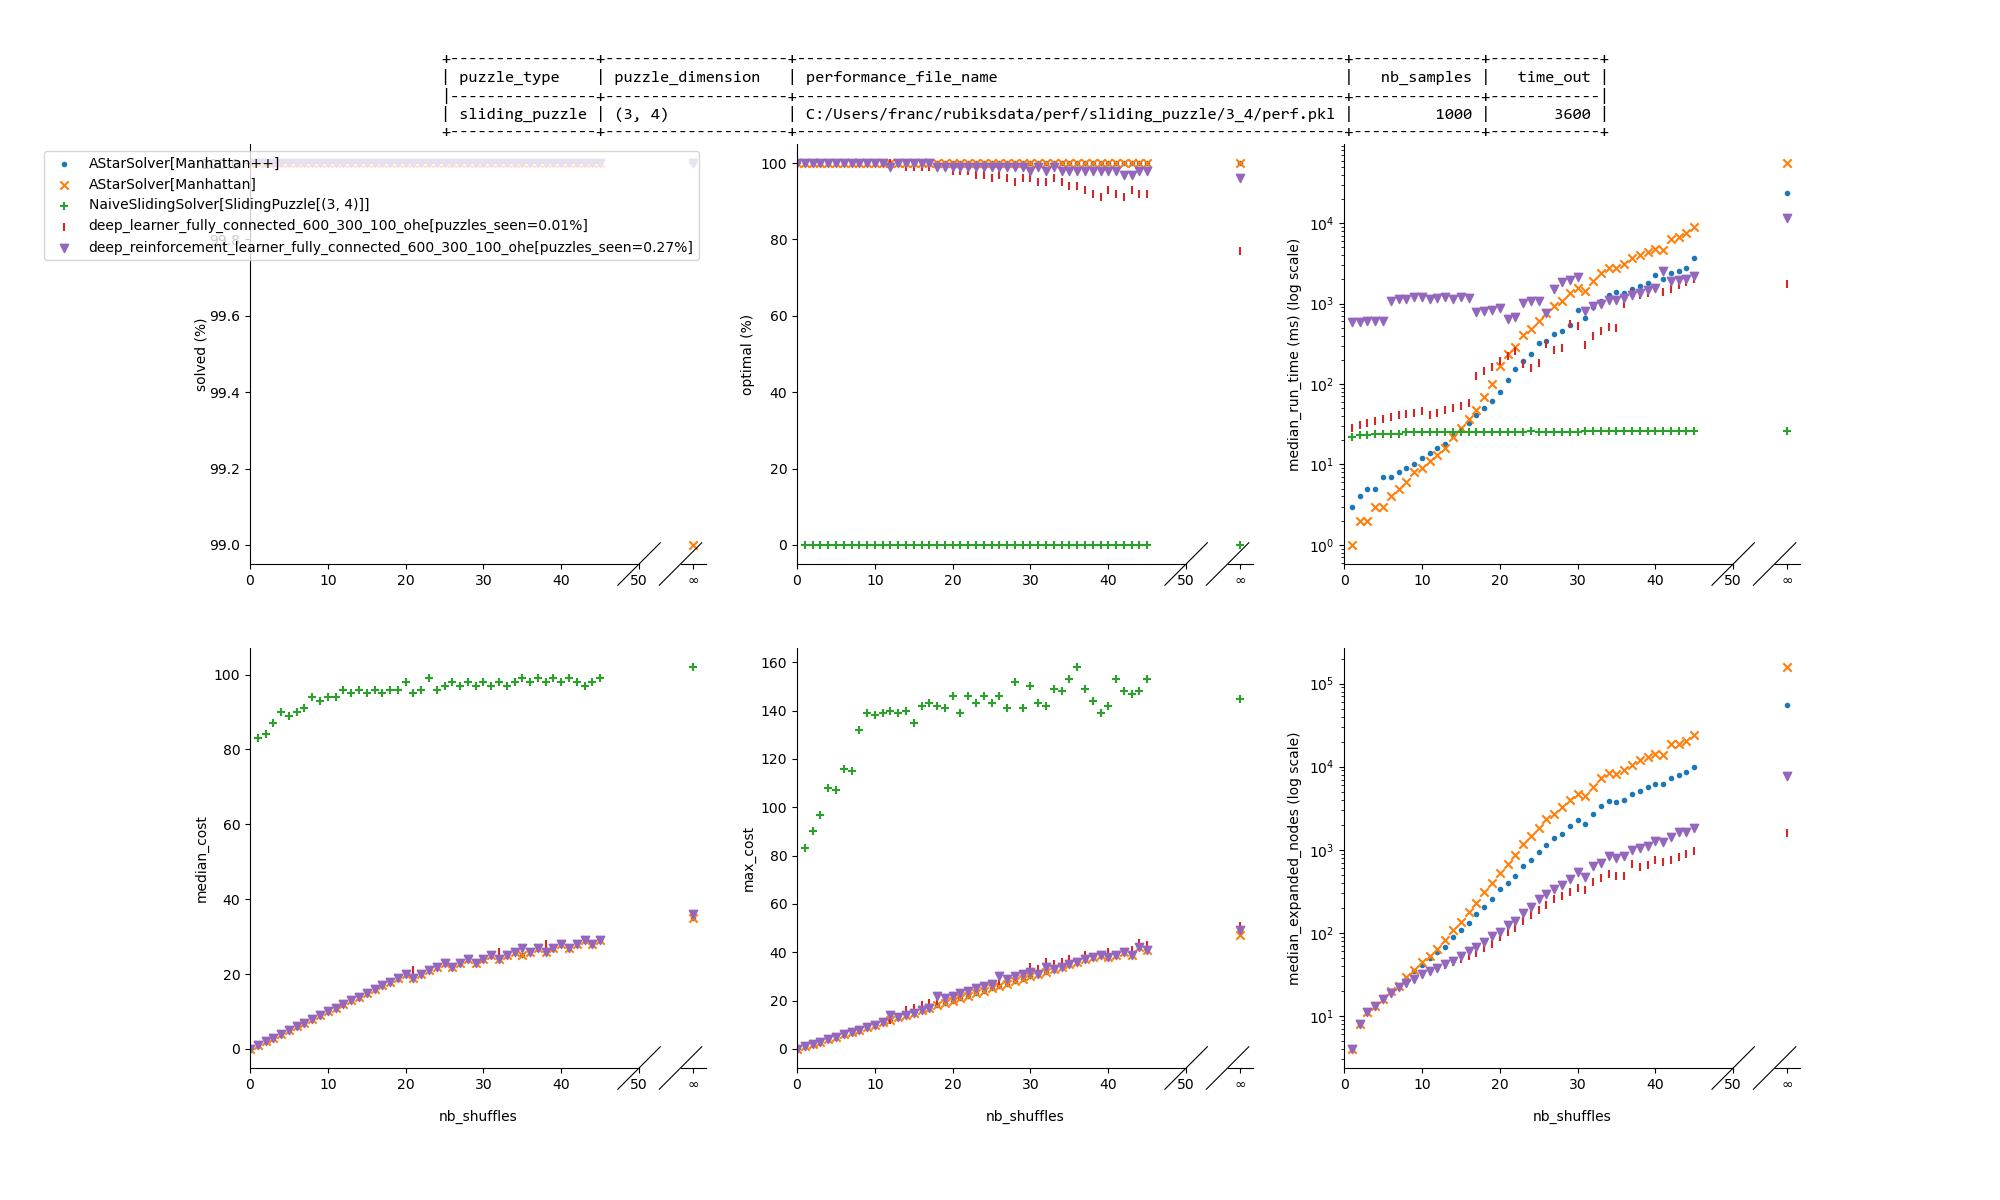
\includegraphics[scale=0.55]{./Figures/34SPPerformance}}
  \caption[34SPPerformance]{Solvers' performance comparison 3x4 \textbf{SP}}
   \label{fig:34SPPerformance}
\end{figure}





%-----------------------------------
%	SECTION 4
%-----------------------------------

\Section{4x4}

In the 4x4 case, due to time constraints, I ran the performance test with 100 random puzzles for difficulty going from 5 to 60 except for $\infty$ shuffling where I only ran a handful of configurations (5). I ran the Naive solver as well as A$^{*}$ with Manhattan++, \textbf{DRL} and \textbf{DL} heuristics, again using the same fully-connected network architecture (left-hand-side of figure \ref{fig:33SPnets}). The 4x4 \textbf{SP} has 10,461,394,944,000 total possible configurations so it does start being quite a large state space! Again \textbf{DL} got trained on randomly generated configurations solved by A$^{*}$[Manhattan++]. \textbf{DL} obtained an optimality scores of 97\%+ across all levels of difficulty and \textbf{DRL} managed 99\%+. \textbf{DL} and \textbf{DRL} saw of the order of respectively $10^{-7}$\% and $10^{-5}$\% of all configurations during training, so again showed impressive performance and generalization!


\label{ssec:44SPSC}

\begin{figure}[H]
  \noindent
  \makebox[\textwidth]{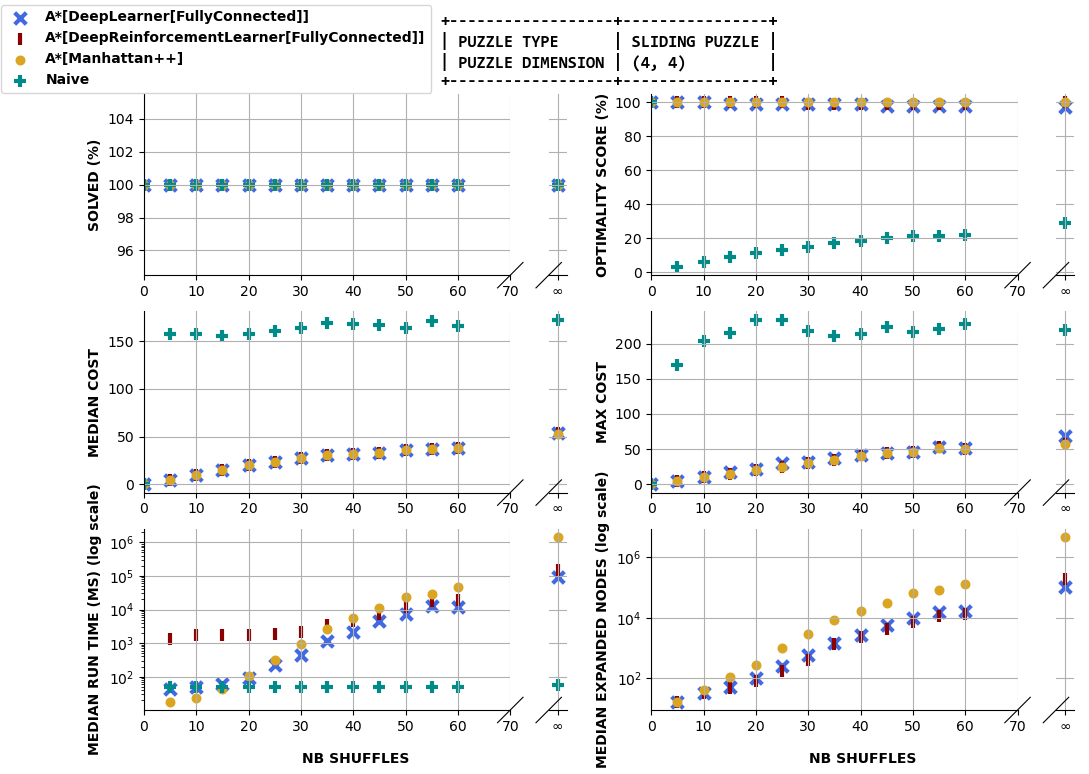
\includegraphics[scale=0.6]{./Figures/44SPPerformance}}
  \caption[44SPPerformance]{Solvers' performance comparison 4x4 \textbf{SP}}
  \label{fig:44SPPerformance}
\end{figure}

